%!TEX program = xelatex
% Full compilation: xelatex → biber/bibtex → xelatex → xelatex
\documentclass[letterpaper,12pt]{article}


% 添加中文支持
\usepackage[UTF8]{ctex} % 这是添加中文支持的关键

\usepackage{fullpage} % Package to use full page
\usepackage{parskip} % Package to tweak paragraph skipping
\usepackage{tikz} % Package for drawing
\usepackage{mathtools}
\usepackage{amsfonts}
\usepackage{fancyhdr}
\usepackage{times}
\usepackage{changepage}
\usepackage{amssymb}
\usepackage{amsthm}
%\usepackage[english]{babel}
\usepackage{graphicx}
\usepackage{xr-hyper}
\usepackage{hyperref}
%\theoremstyle{plain}

\newtheorem{theorem}{Theorem}
\newtheorem{lemma}{Lemma}
\newtheorem{assumption}{Assumption}

\def\mathbi#1{\textbf{\em #1}}

\newcommand{\bsa}{\boldsymbol{a}}
\newcommand{\bsb}{\boldsymbol{b}}
\newcommand{\bsc}{\boldsymbol{c}}
\newcommand{\bsd}{\boldsymbol{d}}
\newcommand{\bse}{\boldsymbol{e}}
\newcommand{\bsf}{\boldsymbol{f}}
\newcommand{\bsg}{\boldsymbol{g}}
\newcommand{\bsh}{\boldsymbol{h}}
\newcommand{\bsi}{\boldsymbol{i}}
\newcommand{\bsj}{\boldsymbol{j}}
\newcommand{\bsk}{\boldsymbol{k}}
\newcommand{\bsl}{\boldsymbol{l}}
\newcommand{\bsm}{\boldsymbol{m}}
\newcommand{\bsn}{\boldsymbol{n}}
\newcommand{\bso}{\boldsymbol{o}}
\newcommand{\bsp}{\boldsymbol{p}}
\newcommand{\bsq}{\boldsymbol{q}}
\newcommand{\bsr}{\boldsymbol{r}}
\newcommand{\bss}{\boldsymbol{s}}
\newcommand{\bst}{\boldsymbol{t}}
\newcommand{\bsu}{\boldsymbol{u}}
\newcommand{\bsv}{\boldsymbol{v}}
\newcommand{\bsw}{\boldsymbol{w}}
\newcommand{\bsx}{\boldsymbol{x}}
\newcommand{\bsy}{\boldsymbol{y}}
\newcommand{\bsz}{\boldsymbol{z}}

\newcommand{\bsA}{\boldsymbol{A}}
\newcommand{\bsB}{\boldsymbol{B}}
\newcommand{\bsC}{\boldsymbol{C}}
\newcommand{\bsD}{\boldsymbol{D}}
\newcommand{\bsE}{\boldsymbol{E}}
\newcommand{\bsF}{\boldsymbol{F}}
\newcommand{\bsG}{\boldsymbol{G}}
\newcommand{\bsH}{\boldsymbol{H}}
\newcommand{\bsI}{\boldsymbol{I}}
\newcommand{\bsJ}{\boldsymbol{J}}
\newcommand{\bsK}{\boldsymbol{K}}
\newcommand{\bsL}{\boldsymbol{L}}
\newcommand{\bsM}{\boldsymbol{M}}
\newcommand{\bsN}{\boldsymbol{N}}
\newcommand{\bsO}{\boldsymbol{O}}
\newcommand{\bsP}{\boldsymbol{P}}
\newcommand{\bsQ}{\boldsymbol{Q}}
\newcommand{\bsR}{\boldsymbol{R}}
\newcommand{\bsS}{\boldsymbol{S}}
\newcommand{\bsT}{\boldsymbol{T}}
\newcommand{\bsU}{\boldsymbol{U}}
\newcommand{\bsV}{\boldsymbol{V}}
\newcommand{\bsW}{\boldsymbol{W}}
\newcommand{\bsX}{\boldsymbol{X}}
\newcommand{\bsY}{\boldsymbol{Y}}
\newcommand{\bsZ}{\boldsymbol{Z}}



\newcommand{\bsigma}{\boldsymbol{\sigma}}
\newcommand{\bsPhi}{\boldsymbol{\Phi}}
\newcommand{\bsphi}{\boldsymbol{\phi}}
\newcommand{\bstau}{\boldsymbol{\tau}}

\newcommand{\sym}[1]{\operatorname{sym}#1}
\newcommand{\skw}[1]{\operatorname{skw}#1}
\newcommand{\diver}{\mathop{\mathrm{div}}}
\newcommand{\grad}[1]{\operatorname{grad}#1}
\newcommand{\curl}[1]{\operatorname{curl}#1}
\newcommand{\tr}[1]{\operatorname{tr}#1}
\newcommand{\dev}[1]{\operatorname{dev}#1}
\newcommand{\sign}[1]{\operatorname{sign}#1}
%\newcommand{\span}[1]{\operatorname{span}#1}


\title{$H(\diver;\,\mathbb{S})$-Conforming Finite Elements for Symmetric Tensors}
%\author{Chunyu Chen \\ School of Mathematics and Computational Science, Xiangtan University}

%\date{\today}

\begin{document}
\maketitle

\tableofcontents

\section{Introduction}\label{sec:intro}

In the mixed finite element method for linear elasticity, the stress tensor $\bsigma$ and the displacement $\bsu$ are approximated in the finite element spaces 
$H(\diver; \mathbb{S})$ and $L^2$, respectively, where $\mathbb{S}$ denotes the space of symmetric tensors. The corresponding discrete spaces $\Sigma_h$ and $V_h$ must satisfy the inf–sup condition, whose validity requires that 
$$
\diver \Sigma_h = V_h.
$$

For any simplex $T$, define the trace-free polynomial space
$$
\mathbb{B}_k(\diver, T) := \left\{ \sigma \in \mathbb{P}_k(T, \mathbb{S}) \;\middle|\; \sigma|_{\partial T} \cdot \bsn = 0 \right\}.
$$
It holds that
$$
\diver \mathbb{B}_k(\diver, T) = \mathbb{P}_{k-1}(T, \mathbb{S}) \cap RM^{\perp},
$$
where $RM^{\perp}$ is the $L^2$-orthogonal complement of 
$$
RM := \mathbb{P}_0(T, \mathbb{R}^d) + \mathbb{P}_0(T, \mathbb{K})\bsx,
$$ 
and $\mathbb{K}$ denotes the space of $d$-dimensional skew-symmetric matrices.

Given a simplicial mesh $\mathcal{T}_h$, and an $H(\diver, \mathbb{S})$-conforming finite element space $\Sigma_h$ defined on $\mathcal{T}_h$, we make the following assumptions:
\begin{enumerate}
    \item[(A1)]\label{assumption1prim} For every $T \in \mathcal{T}_h$, we have
    $$
    \diver \Sigma_T = \mathbb{P}_{k-1}(T, \mathbb{S}).
    $$
    
    \item[(A2)]\label{assumption2} The following degrees of freedom are linearly independent on $\Sigma_h$: 
    $$
    \mathcal{N}_{F, \bsq}(\bsigma) := \int_{F} (\bsigma \cdot \bsn) \cdot \bsq \, \mathrm{d}S, \quad \forall \bsq \in \mathbb{P}_1 (T, \mathbb{R}^d), \; F \in \Delta_{d-1}\mathcal{T}_h.
    $$
\end{enumerate}

Under these assumptions, we have
$$
\diver \Sigma_h = \mathbb{P}_{k-1}^{-1}(\mathcal{T}_h, \mathbb{S}),
$$
where assumption~\hyperref[assumption2]{(A2)} ensures that
$$
\prod_{T \in \mathcal{T}_h} RM(T) \subseteq \diver \Sigma_h.
$$

The Hu–Zhang element is an $H(\diver, \mathbb{S})$-conforming finite element whose shape function space is $\mathbb{P}_k(T, \mathbb{S})$. Thus, it automatically satisfies assumption~\hyperref[assumption1prim]{(A1)}. When $k \geq d+1$, it also satisfies assumption~\hyperref[assumption2]{(A2)}. The Hu–Zhang element includes super-smooth degrees of freedom, which enforce normal continuity on all subsimplices of dimension less than or equal to $d-1$. These properties stem from the symmetry and smoothness of the shape function space.

To resolve this issue for $k \leq d$, we enrich the shape function space $\mathbb{P}_k(T, \mathbb{S})$ with additional $H(\diver; \mathbb{S})$-conforming functions. These functions are non-smooth and have nonzero traces $\bsigma \cdot \bsn$ on $\partial T$, thereby ensuring that the degrees of freedom in assumption~\hyperref[assumption2]{(A2)} remain linearly independent. Moreover, to satisfy assumption~\hyperref[assumption1prim]{(A1)}, these functions are required to be divergence-free. We present the construction of these functions below.

\section{Hybridizable $H(\diver; \mathbb{S})$-Conforming Finite Elements}

According to the exactness of the elasticity complex, the functions in $H(\diver; \mathbb{S})$ with zero divergence form the image of the space $U$ under the corresponding differential operator $\mathrm{d}$, where $U$ is the space preceding $H(\diver; \mathbb{S})$ in the elasticity complex:
\begin{equation}
    \label{eq:hilbertcomplex}
    U \xrightarrow{\mathrm{d}} H(\diver; \mathbb{S})
    \xrightarrow{\diver} L^2(\mathbb{R}^d)
\end{equation}
Therefore, one can select functions from the image of $\mathrm{d}$ applied to $U$ as additional basis functions. To construct functions that are not infinitely smooth, we introduce the following split simplex.

\subsection{Split Simplex}

Let $T$ be a $d$-dimensional simplex with $d+1$ vertices denoted by $\bsx_0, \cdots, \bsx_d$. Define:
$$
\bsx_c = \frac{1}{d+1}\sum_{i=0}^d \bsx_i, \quad
\bst_{ij} = \bsx_j - \bsx_i, \quad \bst_{ic} =
\bsx_c - \bsx_i.
$$
For $f \in \Delta(T)$, define $\bst_{fc} = \bst_{f[0]c} = \bsx_c - \bsx_{f[0]}$.

By connecting $\bsx_c$ with each vertex $\bsx_i$, the simplex $T$ is split into $d+1$ $d$-simplices, denoted collectively as $T^R$. Denote by $T_i$ the sub-simplex in $T^R$ that does not contain vertex $\bsx_i$. For each face $f \in \Delta_{d-1} T$, let $T_{f^*}$ denote the sub-simplex that contains $f$. Let $\chi_{T_i}$ be the characteristic function on $T_i$.

\begin{figure}[h]
\centering
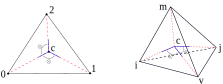
\includegraphics[width=0.7\textwidth]{./figures/splite_cell.pdf}
\caption{Split simplex}
\end{figure}

Define $\lambda_i$ as a continuous piecewise linear function on $T^R$ such that
$$
\lambda_i(\bsx_j) = \delta_{ij}, \quad \forall j = 0, \cdots, d, \quad 
\text{ and } \quad \lambda_i(\bsx_c) = 0.
$$

\begin{lemma}
\label{lem:dual}
For any tetrahedron $T_i$ in $T^R$, with $0\leq i \leq d$, the vectors 
$\{\bst_{cm}\}_{m=0,\, m\ne i}^d$ form a basis of $\mathbb{R}^d$, and 
$\{\nabla \lambda_{m}|_{T_i}\}_{m=0,\, m\ne i}^d$ is the dual basis to it.
\end{lemma}

\section{Mixed Finite-Element Method for Linear Elasticity}\label{sec:mixed}
Let $\Omega\subset\mathbb{R}^d$ ($d=2,3$) be a polygonal domain with boundary $\partial\Omega$.
We study the boundary-value problem
\[
\begin{cases}
\mathcal{A}(\bsigma)=\varepsilon(\bsu) & \text{in }\Omega,\\
\diver\bsigma=\bsf & \text{in }\Omega,\\
\bsu=\mathbf{0} & \text{on }\partial\Omega,
\end{cases}
\]
where $\bsigma$ is the stress tensor, $\bsu$ is the displacement vector,
and $\bsf$ is the body force.
The strain tensor and the compliance tensor are given by
\[
\varepsilon(\bsu)=\tfrac12\bigl(\nabla\bsu+\nabla\bsu^{\mathsf{T}}\bigr),\qquad
\mathcal{A}(\bsigma)=\tfrac1{2\mu}\bigl(\bsigma-\lambda_0\tr\bsigma\,I\bigr),
\]
with Lamé parameters $\lambda$, $\mu>0$.
We partition $\Omega$ by a simplicial mesh $\mathcal{T}_h$ and define
finite-element spaces $\Sigma_h$ and $V_h$ as before.
The mixed finite-element scheme reads:
find $(\bsigma_h,\bsu_h)\in\Sigma_h\times V_h$ such that
\[
\begin{aligned}
\bigl(\mathcal{A}\bsigma_h,\boldsymbol{\tau}\bigr) - \bigl(\diver\boldsymbol{\tau},\bsu_h\bigr) &=0
	&&\forall \boldsymbol{\tau}\in\Sigma_h,\\
\bigl(\diver\bsigma_h,\bsv\bigr) &=\bigl(\bsf,\bsv\bigr)
	&&\forall \bsv\in V_h.
\end{aligned}
\]

\subsection{Two-Dimensional Case}

In two dimensions, the space $U$ in the elasticity complex is $H^2$, and the differential operator $\mathrm{d} = J$ is defined by:
\begin{equation}
\label{eq:Jdef}
J(u) = 
\begin{pmatrix}
  0 & -1\\ 1 & 0
\end{pmatrix}
\nabla^2 u 
\begin{pmatrix}
  0 & 1\\ -1 & 0
\end{pmatrix}
\end{equation}

We now define $H^2$-conforming functions on the split triangle $T^R$. Let the three vertices be $\bsx_0, \bsx_1, \bsx_2$. For vertex \textsf{v}, let $[i, j] = v^*$ (the opposite edge). Define
$$
\psi_{v} = \lambda_v^3 \lambda_i \chi_{T_j} - \lambda_v^3 \lambda_j \chi_{T_i}.
$$

\begin{lemma}
$\psi_v \in H^2(T^R)$.
\end{lemma}
\begin{proof}
It suffices to prove that $\nabla\psi_v$ is continuous across $T^R$, i.e., the jump across each edge $[v, c]$, $[i, c]$, and $[j, c]$ is zero.
\[
\nabla \psi_v = 
(3\lambda_v^2\lambda_i \nabla \lambda_v + \lambda_v^3 \nabla \lambda_i)
\chi_{T_j} -
(3\lambda_v^2\lambda_j \nabla \lambda_v + \lambda_v^3 \nabla \lambda_j)
\chi_{T_i}.
\]
Since $\lambda_v$ vanishes on $[i, c]$ and $[j, c]$, the jump across these two edges is zero. On $[v, c]$, both $\lambda_i$ and $\lambda_j$ vanish, so
\[
[\![\nabla \psi_v]\!]|_{[v, c]} = \lambda_v^3 (\nabla \lambda_i + \nabla \lambda_j).
\]
Because $T_i$ and $T_j$ have equal area, $\nabla \lambda_i$ and $\nabla \lambda_j$ are equal in magnitude but opposite in direction. Hence the jump is zero on $[v, c]$, and the lemma follows.
\end{proof}

Clearly, $\psi_v$ is linearly independent of $\mathbb{P}_k(T, \mathbb{S})$. We further have the following:

\begin{lemma}
\label{lem:jump}
There does not exist $\bsq \in \mathbb{P}_k(T, \mathbb{S})$ such that 
$(\bsq - J(\psi_v))|_{\partial T}\cdot \bsn = 0$.
\end{lemma}
\begin{proof}
$J(\psi_v)$ is discontinuous across $T^R$:
\[
J(\psi_v) : (\bst_{cv}\otimes \bst_{cv}) = 
\nabla^2 \psi_v : (\bsn_{cv}\otimes \bsn_{cv}) = 
\frac{\partial^2 \psi_v}{\partial n_{cv}^2}.
\]
Since $\psi_v$ has a discontinuous second normal derivative across $[v, c]$, we conclude that
$J(\psi_v)|_{T_i} : (\bst_{ci}\otimes \bst_{ci})$ and 
$J(\psi_v)|_{T_j} : (\bst_{cj}\otimes \bst_{cj})$ differ at $\bsx_v$.
Thus $J(\psi_v)\cdot \bsn$ is discontinuous on $\partial T$.

If there exists $\bsq \in \mathbb{P}_k(T, \mathbb{S})$ such that 
$(\bsq - J(\psi_v))\cdot \bsn = 0$ on $\partial T$, then $\bsq$ would also be discontinuous on $\partial T$, which is impossible. The lemma is proved.
\end{proof}

\begin{theorem}
\label{thm:hdivsdof2d}
Define
$$
\Sigma_T = \mathbb{P}_k(T, \mathbb{S}) + \mathrm{span}\{J(\psi_i)\}_{i=0}^2.
$$
Then $\Sigma_T \subset H(\diver; \mathbb{S})$, and the following degrees of freedom are unisolvent:
\begin{align}
(\bsigma\cdot \bsn, \bsq)  & \quad \forall e \in \Delta_1 T,\; \bsq \in \mathbb{P}_k(T, \mathbb{R}^2), \label{eq:dof1}\\
(\bsigma : \bsq) & \quad \forall \bsq \in \mathbb{B}_k(\diver; T). \label{eq:dof2}
\end{align}
\end{theorem}
\begin{proof}
The $H(\diver; \mathbb{S})$-conformity is clear. We now prove unisolvency of the degrees of freedom.

First, count the degrees of freedom. The first kind contributes $6(k+1)$ DOFs. Using geometric decomposition, the second kind contributes
\[
\dim\left(\mathbb{B}_k(\diver; T)\right) = \frac{3(k-1)(k-2)}{2} + 3(k-1).
\]
The total dimension of the space $\Sigma_T$ is 
\[
\dim(\mathbb{P}_k(T, \mathbb{S})) + 3 = \frac{3(k+1)(k+2)}{2} + 3.
\]
A direct computation shows this equals the total number of DOFs.

Now let $\bsigma \in \Sigma_T$ with all DOFs zero. Since $\bsigma\cdot \bsn \in \mathbb{P}_k(T, \mathbb{R}^2)$, the vanishing of the DOFs in \eqref{eq:dof1} implies 
$\bsigma \cdot \bsn|_{\partial T} = 0$, hence $\bsigma \in \mathbb{B}_k(\diver; T)$ by Lemma~\ref{lem:jump}. Then \eqref{eq:dof2} implies $\bsigma = 0$, proving unisolvency.
\end{proof}

Define the global finite element space:
$$
\Sigma_h := \left\{
\bsigma \in L^2(\Omega) \;\middle|\;
\bsigma|_T \in \Sigma_T \text{ for all } T \in \mathcal{T}_h,\;
\text{and DOFs \eqref{eq:dof1} are single-valued}
\right\}.
$$
Then $\Sigma_h$ is an $H(\diver; \mathbb{S})$-conforming finite element space.


\subsection{Arbitrary Dimensional Case}

While the complex-based approach allows extension to arbitrary dimensions, the elasticity complex in dimensions higher than 2 is technically involved. In this section, we present an alternative constructive approach.

We begin by examining the structure of the function $J(\psi_v)$ introduced in the 2D case. Define the rotated gradient
$$
\nabla^{\perp}f = \begin{pmatrix}
-\frac{\partial f}{\partial y} \\ \frac{\partial f}{\partial x}
\end{pmatrix}
= 
\begin{pmatrix}
0 & -1\\ 1 & 0
\end{pmatrix} \nabla f.
$$
Then by the definition of $J$ in \eqref{eq:Jdef}, we have
\begin{align*}
J(\psi_v) =\; & 6\bigl(\lambda_v^2 \sym(\nabla^{\perp} \lambda_i \otimes \nabla^{\perp} \lambda_v) + \lambda_v \lambda_i \nabla^{\perp} \lambda_v \otimes \nabla^{\perp} \lambda_v\bigr) \chi_{T_j}\\
& - 6\bigl(\lambda_v^2 \sym(\nabla^{\perp} \lambda_j \otimes \nabla^{\perp} \lambda_v) + \lambda_v \lambda_j \nabla^{\perp} \lambda_v \otimes \nabla^{\perp} \lambda_v\bigr) \chi_{T_i}.
\end{align*}

Note that there exist constants $c_1, c_2$ such that
$$
\nabla^{\perp} \lambda_v = c_1 \bst_{ci} \chi_{T_j} + c_2 \bst_{cj} \chi_{T_i}.
$$

Let us define:
\begin{align*}
\psi_v^0 &= \lambda_v \lambda_i (\bst_{ci} \otimes \bst_{ci}) \chi_{T_j}, \quad
\psi_v^1 = \lambda_v \lambda_j (\bst_{cj} \otimes \bst_{cj}) \chi_{T_i},\\
\psi_v^2 &= \lambda_v^2 \bigl(\sym(\bst_{cv} \otimes \bst_{ci}) \chi_{T_j} - \sym(\bst_{cv} \otimes \bst_{cj}) \chi_{T_i}\bigr).
\end{align*}
Then $J(\psi_v)$ is a linear combination of $\psi_v^0$, $\psi_v^1$, and $\psi_v^2$.

\begin{lemma}
\label{lem:diver}
The functions $\psi_v^0, \psi_v^1, \psi_v^2$ defined above belong to $H(\diver; \mathbb{S})$, and there exists a linear combination of them whose divergence is zero.
\end{lemma}

\begin{proof}
We only need to verify normal continuity across the internal edges $[v, c]$, $[i, c]$, and $[j, c]$. The functions $\psi_v^0$ and $\psi_v^1$ vanish on these edges. $\psi_v^2$ vanishes on $[i, c]$ and $[j, c]$, and on $[v, c]$ we compute
\[
[\![\psi_v^2 \cdot \bsn_{[v,c]}]\!] = \frac{1}{2} \lambda_v^2 ((\bst_{ci} + \bst_{cj}) \cdot \bsn_{[v, c]}) \bst_{cv}.
\]
Since
\[
\bst_{ci} + \bst_{cj} = \bsx_c - \bsx_i + \bsx_c - \bsx_j = \bsx_v - \bsx_c = -\bst_{cv},
\]
the jump vanishes, establishing $H(\diver; \mathbb{S})$-conformity.

Next, compute the divergence:
\[
\diver(\psi_v^0) = \lambda_v \bst_{ci} \chi_{T_j}, \quad 
\diver(\psi_v^1) = \lambda_v \bst_{cj} \chi_{T_i}, \quad 
\diver(\psi_v^2) = \lambda_v (\bst_{ci} \chi_{T_j} - \bst_{cj} \chi_{T_i}).
\]
Thus,
\[
\diver(\psi_v^2 - \psi_v^0 + \psi_v^1) = 0.
\]
\end{proof}

The lemma shows that we can construct the desired functions in a constructive manner. The key is to use tensor products of vectors from $\{\bst_{c0}, \bst_{c1}, \ldots, \bst_{cd}\}$, which are dual to $\{\nabla \lambda_0, \nabla \lambda_1, \ldots, \nabla \lambda_d\}$ as shown in Lemma~\ref{lem:dual}, simplifying divergence calculations. We now generalize this to arbitrary dimensions.

Let $T$ be a $d$-simplex, and let $e$ be an $l$-face of $T$ with $l < d-1$. For $\alpha \in \mathbb{T}_k^l$, define the monomial
$$
\lambda_e^\alpha = \lambda_{e[0]}^{\alpha_0} \lambda_{e[1]}^{\alpha_1} \cdots \lambda_{e[l]}^{\alpha_l}.
$$

We define three types of $H(\diver; \mathbb{S})$-conforming functions as in the 2D case. For $\alpha \in \mathring{\mathbb{T}}_k^l := \{\alpha \in \mathbb{T}_k^l \mid \alpha_i \ne 0,\; \forall i\}$ and $i<j \in e^*$, define
\begin{align*}
\psi_{ij,0}^{e,\alpha} &= \lambda_e^{\alpha - \epsilon_0} \lambda_i\, \bst_{ci} \otimes \bst_{ci}\, \chi_{T_j},\\
\psi_{ij,1}^{e,\alpha} &= \lambda_e^{\alpha - \epsilon_0} \lambda_j\, \bst_{cj} \otimes \bst_{cj}\, \chi_{T_i},\\
\psi_{ij,2}^{e,\alpha} &= \lambda_e^{\alpha} \bigl(\sym(\bst_{ce} \otimes \bst_{ci}) \chi_{T_j} - \sym(\bst_{ce} \otimes \bst_{cj}) \chi_{T_i}\bigr),
\end{align*}
where $\epsilon_0 = (1, 0, \ldots, 0)$ is a vector of length $l+1$.

\begin{lemma}
\label{lem:diver2}
For all $\alpha \in \mathring{\mathbb{T}}_k^l$ and $i<j \in e^*$, the functions $\psi_{ij,0}^{e,\alpha}, \psi_{ij,1}^{e,\alpha}, \psi_{ij,2}^{e,\alpha}$ belong to $H(\diver; \mathbb{S})$, and there exists a linear combination whose divergence vanishes.
\end{lemma}

\begin{proof}
Let $\bar{f} = f \cup \{\bsx_c\} \in \Delta \mathring{T^R}$ denote an interior face of $T^R$. We verify normal continuity across each $\bar{f}$ for $f \in \Delta_{d-2}T$.

For $\psi_{ij,0}^{e,\alpha}$, if $\bar{f} \notin \Delta_{d-1} T_j$, the function vanishes on $\bar{f}$. If $q = T_j \setminus \bar{f} = i$, then $\lambda_i$ vanishes on $\bar{f}$. If $q \ne i$, then $\nabla \lambda_q$ is normal to $\bar{f}$ and orthogonal to $\bst_{ci}$ by Lemma~\ref{lem:dual}, so the normal component of $\psi_{ij,0}^{e,\alpha}$ vanishes. Similar arguments apply to $\psi_{ij,1}^{e,\alpha}$.

For $\psi_{ij,2}^{e,\alpha}$, the only nontrivial case is when $f = [i,j]^*$. In that case, choosing $\bsn_{\bar{f}} = \nabla \lambda_i|_{T_j}$ and noting
\[
\bst_{ci} + \bst_{cj} = -\bst_{ce}, \quad 
\nabla \lambda_i|_{T_j} \cdot \bst_{ci} = 1, \quad 
\nabla \lambda_j|_{T_i} \cdot \bst_{cj} = 1,
\]
we compute
\[
[\![\psi_{ij,2}^{e,\alpha} \cdot \bsn_{\bar{f}}]\!] = \frac{1}{2} \lambda_e^\alpha\, (\bst_{ci} + \bst_{cj}) \cdot \nabla \lambda_i \, \bst_{ce} = 0.
\]

The divergence is:
\begin{align*}
\diver(\psi_{ij,0}^{e,\alpha}) &= \lambda_e^{\alpha - \epsilon_0} \bst_{ci} \chi_{T_j},\\
\diver(\psi_{ij,1}^{e,\alpha}) &= \lambda_e^{\alpha - \epsilon_0} \bst_{cj} \chi_{T_i},\\
\diver(\psi_{ij,2}^{e,\alpha}) &= \frac{\alpha_0}{2} \lambda_e^{\alpha - \epsilon_0} (\bst_{ci} \chi_{T_j} - \bst_{cj} \chi_{T_i}).
\end{align*}
Let
\[
\psi_{ij}^{e,\alpha} = -\frac{\alpha_0}{2} \psi_{ij,0}^{e,\alpha} + \frac{\alpha_0}{2} \psi_{ij,1}^{e,\alpha} + \psi_{ij,2}^{e,\alpha}.
\]
Then $\diver(\psi_{ij}^{e,\alpha}) = 0$.
\end{proof}

\begin{lemma}
\label{lem:jump}
There does not exist $\bsq \in \mathbb{P}_k(T, \mathbb{S})$ such that 
\[
(\bsq - \psi_{ij}^{e,\alpha})\cdot \bsn = 0 \quad \text{on } \partial T.
\]
\end{lemma}
\begin{proof}
The proof is similar to Lemma~\ref{lem:jump} in the 2D case.
\end{proof}

\begin{theorem}
\label{thm:hdivsdofnd}
Let
\[
V_T := \mathbb{P}_k(T, \mathbb{S}) \oplus \bigoplus_{l=0}^{d-2} \bigoplus_{e \in \Delta_l T} \mathrm{span}(\Phi_e^k),
\]
where
\[
\Phi_e^k = \left\{ \psi_{ij}^{e,\alpha} \mid i<j \in e^*,\; \alpha \in \mathring{\mathbb{T}}_k^l \right\}.
\]
Then $V_T \subset H(\diver; \mathbb{S})$, and the following degrees of freedom are unisolvent:
\begin{align}
(\bsigma\cdot \bsn, \bsq)_F & \quad \forall F \in \Delta_{d-1} T,\; \bsq \in \mathbb{P}_k(F, \mathbb{R}^d), \label{eq:dof3}\\
(\bsigma : \bsq)_T & \quad \forall \bsq \in \mathbb{B}_k(\diver; T). \label{eq:dof4}
\end{align}
\end{theorem}

\begin{proof}
The proof is analogous to that of Theorem~\ref{thm:hdivsdof2d}.
\end{proof}

Define the global finite element space
\[
\Sigma_h := \left\{ \bsigma \in L^2(\Omega) \;\middle|\;
\bsigma|_T \in V_T,\; \forall T \in \mathcal{T}_h,\;
\text{and DOFs \eqref{eq:dof3} are single-valued} \right\}.
\]

\begin{theorem}
\label{thm:infsup}
We have $\diver \Sigma_h = \mathbb{P}_{k-1}^{-1}(\mathcal{T}_h, \mathbb{S})$, and there exists a constant $C > 0$ such that
\begin{equation}
\label{eq:infsup}
\sup_{\bstau \in \Sigma_h} 
\frac{(\diver \bstau, \bsv)}{\|\bstau\|_{H(\diver)}}
\geq C \|\bsv\|_{L^2}.
\end{equation}
\end{theorem}

\begin{proof}
[Proof omitted.]
\end{proof}


\section{Numerical Experiments}

\subsection{Mixed Finite Element Method for Linear Elasticity}

Let $\Omega \subset \mathbb{R}^d$ ($d = 2, 3$) be a polygonal domain with boundary $\partial \Omega$. We consider the linear elasticity problem:
\begin{equation*}
\left\{
\begin{aligned}
  \mathcal{A}(\bsigma) - \varepsilon(\bsu) & = 0, \quad \text{in } \Omega, \\
  -\diver \bsigma &= \bsf, \quad \text{in } \Omega, \\
  \bsu &= 0, \quad \text{on } \partial \Omega,
\end{aligned}
\right.
\end{equation*}
where $\bsigma$ is the stress tensor, $\bsu$ is the displacement vector, and $\bsf$ is the body force. The strain tensor $\varepsilon(\bsu)$ and the compliance operator $\mathcal{A}(\bsigma)$ are defined as:
\[
\varepsilon(\bsu) = \tfrac{1}{2}(\nabla \bsu + \nabla \bsu^{\mathsf{T}}), \quad
\mathcal{A}(\bsigma) = \lambda_0 \bsigma - \lambda_1 \operatorname{tr}(\bsigma) I.
\]
Here, $\lambda$ and $\mu$ are the Lamé constants, and the coefficients are given by
\[
\lambda_0 = \frac{1}{2\mu}, \quad
\lambda_1 = \frac{\lambda}{2\mu(2\mu + d\lambda)},
\]
where $I$ denotes the identity tensor.

Let $\mathcal{T}_h$ be a simplicial mesh of $\Omega$, and define the discrete stress space $\Sigma_h$ and displacement space $V_h := \mathbb{P}_{k-1}^{-1}(\mathcal{T}_h)$. The mixed finite element method for the linear elasticity system seeks $(\bsigma_h, \bsu_h) \in \Sigma_h \times V_h$ such that:
\begin{equation}
\begin{aligned}
    a(\bsigma_h, \bstau_h) + b(\bstau_h, \bsu_h) &= 0, \quad \forall\, \bstau_h \in \Sigma_h, \\
    b(\bsigma_h, \bsv_h) &= (-\bsf, \bsv_h), \quad \forall\, \bsv_h \in V_h,
\end{aligned}
\end{equation}
where the bilinear forms are defined by
\[
a(\bsigma_h, \bstau_h) = (\mathcal{A}(\bsigma_h), \bstau_h), \quad
b(\bstau_h, \bsu_h) = (\diver \bstau_h, \bsu_h).
\]

\subsection{Two-Dimensional Example}

Let the exact solution be given by
\[
\bsu = (\sin(5x)\sin(7y), \cos(5x)\cos(4y)),
\]
on the domain $\Omega = (0,1)^2$, with parameters $\lambda_0 = 4$ and $\lambda_1 = 1$.

Figure~\ref{fig:k235} shows the numerical results for polynomial degrees $k = 2$, $3$, and $5$. The observed convergence rates confirm the theoretical estimates:
\[
\|\bsigma - \bsigma_h\|_{L^2} = O(h^{k+1}), \quad
\|\bsu - \bsu_h\|_{L^2} = O(h^k).
\]



\begin{figure}[htb]
\centering
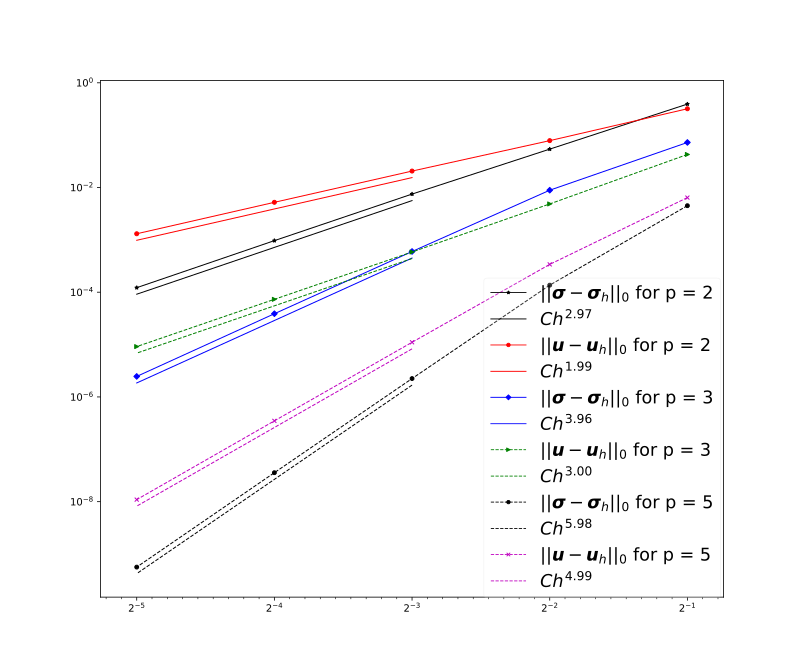
\includegraphics[width=0.9\textwidth]{figures/divs.pdf}
\caption{Convergence results for $k=2,3,5$.}\label{fig:k235}
\end{figure}



\section{Conclusion}
We have constructed a family of $H(\diver,\mathbb{S})$-conforming finite elements
that extend the Hu–Zhang framework to any polynomial degree $k\ge2$.
Under mild assumptions, the discrete divergence operator is onto,
guaranteeing the inf–sup stability of the mixed formulation.
Numerical experiments confirm the optimal convergence orders
predicted by the theory.

\bibliographystyle{plain}
\bibliography{references}

\end{document}
